
\documentclass{standalone}
\usepackage{tikz}
\usetikzlibrary{arrows,positioning}
\tikzset{
    %Define standard arrow tip
    >=stealth',
    %Define style for boxes
    punkt/.style={
           rectangle,
           rounded corners,
           draw=black, thick,
           text width=4.5em,
           minimum height=2em,
           text centered},
    node/.style={
           rectangle,
           rounded corners,
           draw=black, thin,
           text width=3.5em,
           minimum height=2em,
           text centered},
    node/.style={
           rectangle,
           rounded corners,
           draw=black,
           text width=4.5em,
           minimum height=2em,
           text centered,
           fill={rgb:black,1;white,3}},
    % Define arrow style
    pil/.style={
           ->,
           thick,
           shorten <=2pt,
           shorten >=2pt,}
every node/.style={align=center}
}

\begin{document}

\begin{tikzpicture}
\node[scale=0.8] at (-2,0) {
\begin{tikzpicture}[node distance=1cm, auto,]
\node[punkt, text width=6em] (pseudo) at (6.4,-11.8) {closest node};
\node[node] (node3) at (9,-4) {node};
\node[punkt] (retriever) at (10,-1) {retriever}
  edge[pil, ->, bend right=10] node[left=1pt]{retrieval} node[right=1pt]{ request} (node3);
\node[punkt] (custodian) at (5.5,-9) {custodian}
(custodian.-15) edge[pil,dashed, bend left=30, <->] node[right]{
  \begin{tabular}{c}missing\\ link\end{tabular}
  }(pseudo);
\node[node] (node4) at (8,-6) {node}
  (node4.south) edge[pil, ->, bend left=45] node[left=3pt]{failed}node[right=1pt]{ retrieval}(pseudo.east)
  (node4.north) edge[pil,<-,dashed, bend left=15] node[auto]{forwarding}(node3);
\node (chunklabel) at (4,-10) {chunk address};
\node (chunk) at (6,-11) {$\bullet$}
 edge[pil, <-] (chunklabel.south east);
\end{tikzpicture}
};
\node[scale=0.8] at (5,0) {

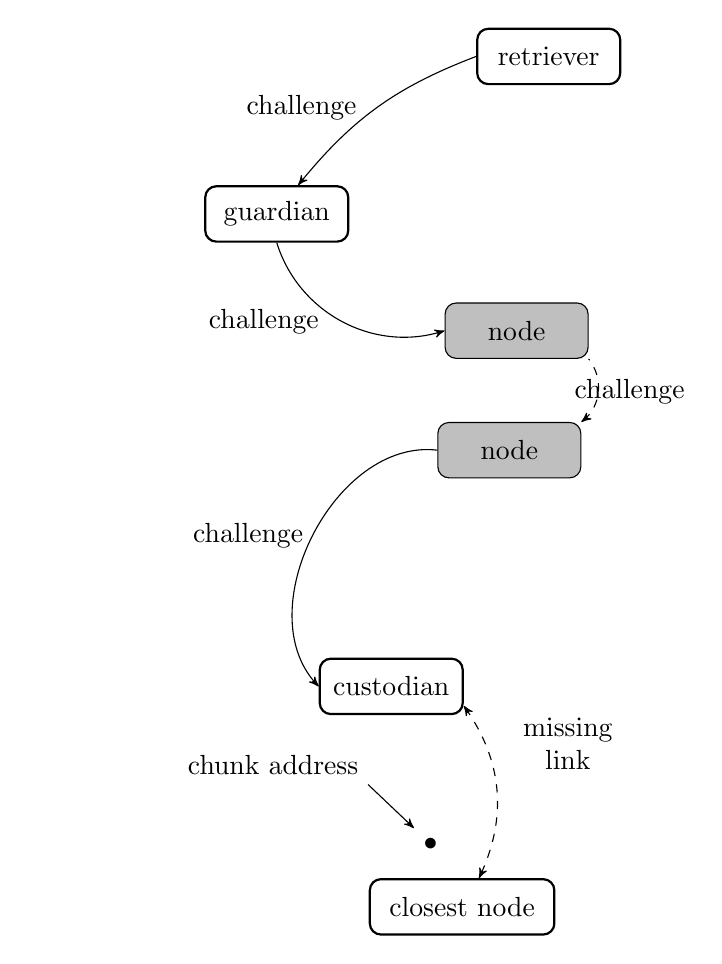
\begin{tikzpicture}[node distance=1cm, auto,]
\node at (-2,0) (owner){};
%guardian, arrow from owner
\node[punkt, right=2cm of owner] (guardian) {guardian};
%node after guardian - arrow to node
\node[right=2cm of guardian] (rog) {};
\node[node, below=of rog] (node1) {node}
  (node1.west) edge[pil, <-, bend left=45] node[left=5pt] {challenge} (guardian.south);
\node[punkt, text width=6em] (pseudo) at (3.4,-8.8) {closest node};
%
\node[node] (node2) at (4,-3) {node}
  (node2.north east) edge[pil, <-, dashed, bend right=45] node[right=-12pt] {challenge} (node1.south east);
\node[punkt] (retriever) at (4.5,2) {retriever};
\node[punkt] (custodian) at (2.5,-6) {custodian}
(custodian.-15) edge[pil,dashed, bend left=30, <->] node[auto]{
  \begin{tabular}{c}missing\\ link\end{tabular}
  }(pseudo)
  (custodian.west) edge[pil, <-, bend left=70] node[left]{challenge} (node2.west);
\node (chunklabel) at (1,-7) {chunk address};
\node (chunk) at (3,-8) {$\bullet$}
 edge[pil, <-] (chunklabel.south east)
 (retriever.west) edge[pil, ->, bend right=15] node[left=4pt]{challenge} (guardian);
\end{tikzpicture}
};
\end{tikzpicture}
\end{document}
